\clearpage


\section{Figures and tables from Part \#1}\label{sec:references-from-part-1}

\subsection{Features from Part \#1}\label{subsec:features-from-part-1}
\begin{table}[!h]
    \resizebox{\textwidth}{!}{
        \begin{tabular}{|l|l|l|}
            \hline
            Feature   & Description                                                  & Reason                                               \\ \hline
            Canvas    & Implement a pixel canvas that will display the current state & Main feature of the website                          \\ \hline
            Websocket & Using websocket protocol to allow for real-time updates      & Give users instant feedback on changes to the canvas \\ \hline
        \end{tabular}
    }
    \caption{Main features}
    \label{tab:mainFeatures}
\end{table}

\begin{table}[!h]
    \resizebox{\textwidth}{!}{
        \begin{tabular}{|l|l|l|}
            \hline
            Feature      & Description                       & Reason                    \\ \hline
            Login system & System to track users             & Potential personalisation \\ \hline
            Timeout      & Restrict canvas editing frequency & Reduce bot behavior       \\ \hline
        \end{tabular}
    }
    \caption{Additional features}
    \label{tab:additionalFeatures}
\end{table}

\subsection{Wireframe}\label{subsec:wireframe3}
\begin{figure}[H]
    \centering
    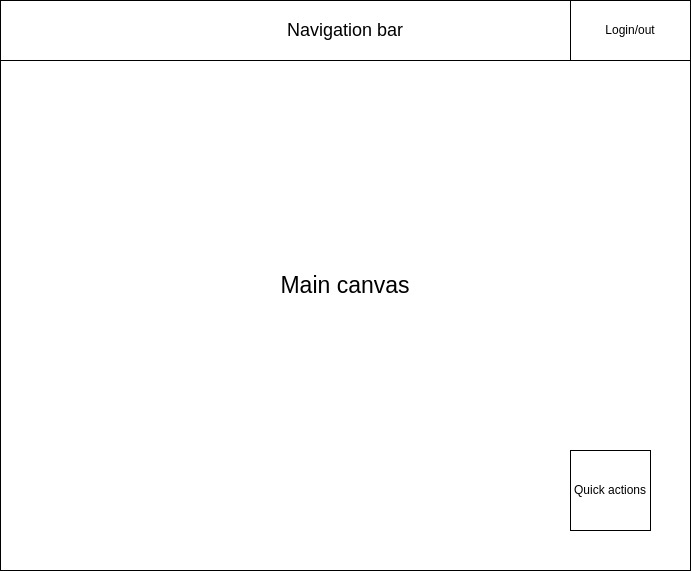
\includegraphics[width=0.8\textwidth]{../images/wireframe}
    \caption{Wireframe for application}
    \label{fig:wireframe}
\end{figure}

\clearpage

\subsection{Navigation tree}\label{subsec:navigation-tree3}
\begin{figure}[h]
    \centering
    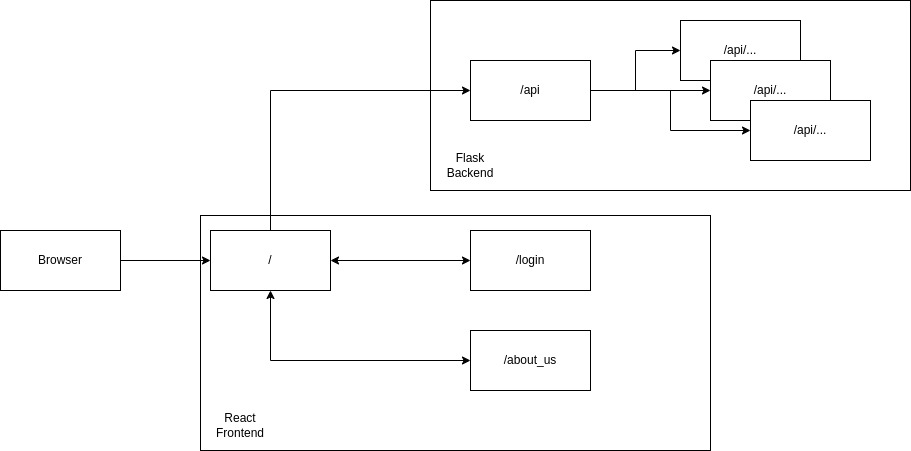
\includegraphics[width=\textwidth]{../images/navigation tree}
    \caption{Navigation tree for single-page React application with Flask backend}
    \label{fig:navigationTree}
\end{figure}


\section{PocketBase screenshots}
\begin{figure}[H]
    \centering
    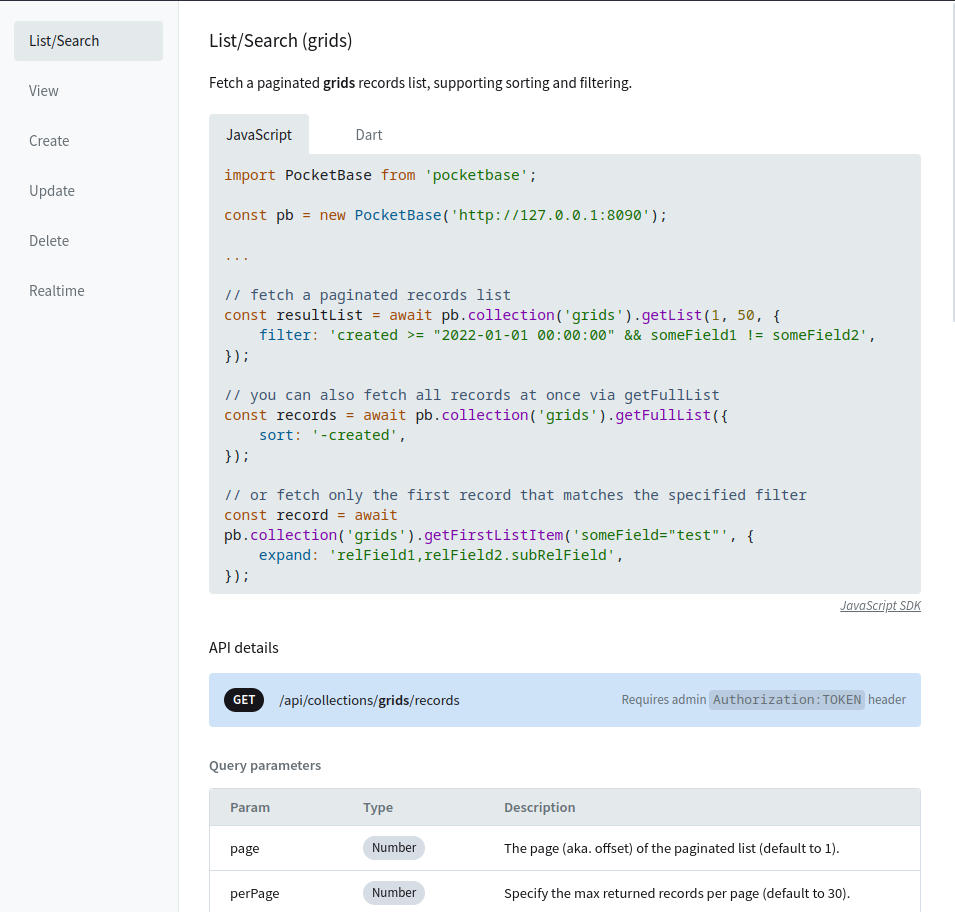
\includegraphics[width=\textwidth + 10]{../images/pbEndpoints}
    \caption{Endpoint preview}
    \label{fig:pbEndpoints}
\end{figure}


\section{Architecture diagram}\label{sec:architecture-diagram}
\begin{figure}[H]
    \centering
    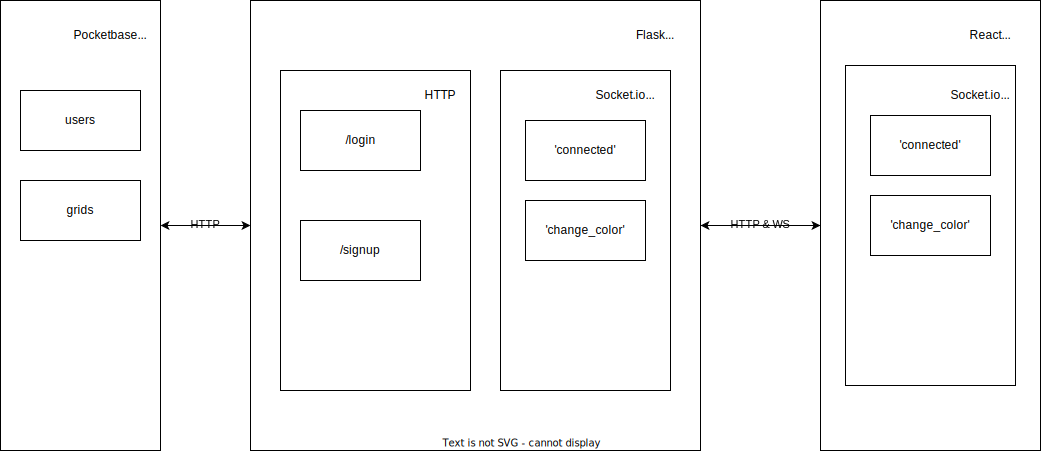
\includegraphics[width=\textwidth + 10]{../images/architecture}
    \caption{Architeture for Squarish}
    \label{fig:architecture}
\end{figure}